\documentclass[11pt,compress,t,notes=noshow, xcolor=table]{beamer}

\documentclass[11pt,compress,t,notes=noshow, xcolor=table]{beamer}
\usepackage[]{graphicx}\usepackage[]{color}
% maxwidth is the original width if it is less than linewidth
% otherwise use linewidth (to make sure the graphics do not exceed the margin)
\makeatletter
\def\maxwidth{ %
  \ifdim\Gin@nat@width>\linewidth
    \linewidth
  \else
    \Gin@nat@width
  \fi
}
\makeatother

\definecolor{fgcolor}{rgb}{0.345, 0.345, 0.345}
\newcommand{\hlnum}[1]{\textcolor[rgb]{0.686,0.059,0.569}{#1}}%
\newcommand{\hlstr}[1]{\textcolor[rgb]{0.192,0.494,0.8}{#1}}%
\newcommand{\hlcom}[1]{\textcolor[rgb]{0.678,0.584,0.686}{\textit{#1}}}%
\newcommand{\hlopt}[1]{\textcolor[rgb]{0,0,0}{#1}}%
\newcommand{\hlstd}[1]{\textcolor[rgb]{0.345,0.345,0.345}{#1}}%
\newcommand{\hlkwa}[1]{\textcolor[rgb]{0.161,0.373,0.58}{\textbf{#1}}}%
\newcommand{\hlkwb}[1]{\textcolor[rgb]{0.69,0.353,0.396}{#1}}%
\newcommand{\hlkwc}[1]{\textcolor[rgb]{0.333,0.667,0.333}{#1}}%
\newcommand{\hlkwd}[1]{\textcolor[rgb]{0.737,0.353,0.396}{\textbf{#1}}}%
\let\hlipl\hlkwb

\usepackage{framed}
\makeatletter
\newenvironment{kframe}{%
 \def\at@end@of@kframe{}%
 \ifinner\ifhmode%
  \def\at@end@of@kframe{\end{minipage}}%
  \begin{minipage}{\columnwidth}%
 \fi\fi%
 \def\FrameCommand##1{\hskip\@totalleftmargin \hskip-\fboxsep
 \colorbox{shadecolor}{##1}\hskip-\fboxsep
     % There is no \\@totalrightmargin, so:
     \hskip-\linewidth \hskip-\@totalleftmargin \hskip\columnwidth}%
 \MakeFramed {\advance\hsize-\width
   \@totalleftmargin\z@ \linewidth\hsize
   \@setminipage}}%
 {\par\unskip\endMakeFramed%
 \at@end@of@kframe}
\makeatother

\definecolor{shadecolor}{rgb}{.97, .97, .97}
\definecolor{messagecolor}{rgb}{0, 0, 0}
\definecolor{warningcolor}{rgb}{1, 0, 1}
\definecolor{errorcolor}{rgb}{1, 0, 0}
\newenvironment{knitrout}{}{} % an empty environment to be redefined in TeX

\usepackage{alltt}
\newcommand{\SweaveOpts}[1]{}  % do not interfere with LaTeX
\newcommand{\SweaveInput}[1]{} % because they are not real TeX commands
\newcommand{\Sexpr}[1]{}       % will only be parsed by R
\newcommand{\xmark}{\ding{55}}%


\usepackage[english]{babel}
\usepackage[utf8]{inputenc}

\usepackage{dsfont}
\usepackage{verbatim}
\usepackage{amsmath}
\usepackage{amsfonts}
\usepackage{amssymb}
\usepackage{bm}
\usepackage{csquotes}
\usepackage{multirow}
\usepackage{longtable}
\usepackage{booktabs}
\usepackage{enumerate}
\usepackage[absolute,overlay]{textpos}
\usepackage{psfrag}
\usepackage{algorithm}
\usepackage{algpseudocode}
\usepackage{eqnarray}
\usepackage{arydshln}
\usepackage{tabularx}
\usepackage{placeins}
\usepackage{tikz}
\usepackage{setspace}
\usepackage{colortbl}
\usepackage{mathtools}
\usepackage{wrapfig}
\usepackage{bm}
\usepackage{amsmath}
\usepackage{pifont}

\usetikzlibrary{shapes,arrows,automata,positioning,calc,chains,trees, shadows}
\tikzset{
  %Define standard arrow tip
  >=stealth',
  %Define style for boxes
  punkt/.style={
    rectangle,
    rounded corners,
    draw=black, very thick,
    text width=6.5em,
    minimum height=2em,
    text centered},
  % Define arrow style
  pil/.style={
    ->,
    thick,
    shorten <=2pt,
    shorten >=2pt,}
}

\usepackage{subfig}

% Defines macros and environments
\usepackage{../../style/lmu-lecture}


\let\code=\texttt
\let\proglang=\textsf

\setkeys{Gin}{width=0.9\textwidth}

\setbeamertemplate{frametitle}{\expandafter\uppercase\expandafter\insertframetitle}

\usepackage{bbm}
% basic latex stuff
\newcommand{\pkg}[1]{{\fontseries{b}\selectfont #1}} %fontstyle for R packages
\newcommand{\lz}{\vspace{0.5cm}} %vertical space
\newcommand{\dlz}{\vspace{1cm}} %double vertical space
\newcommand{\oneliner}[1] % Oneliner for important statements
{\begin{block}{}\begin{center}\begin{Large}#1\end{Large}\end{center}\end{block}}


%new environments
\newenvironment{vbframe}  %frame with breaks and verbatim
{
 \begin{frame}[containsverbatim,allowframebreaks]
}
{
\end{frame}
}

\newenvironment{vframe}  %frame with verbatim without breaks (to avoid numbering one slided frames)
{
 \begin{frame}[containsverbatim]
}
{
\end{frame}
}

\newenvironment{blocki}[1]   % itemize block
{
 \begin{block}{#1}\begin{itemize}
}
{
\end{itemize}\end{block}
}

\newenvironment{fragileframe}[2]{  %fragile frame with framebreaks
\begin{frame}[allowframebreaks, fragile, environment = fragileframe]
\frametitle{#1}
#2}
{\end{frame}}


\newcommand{\myframe}[2]{  %short for frame with framebreaks
\begin{frame}[allowframebreaks]
\frametitle{#1}
#2
\end{frame}}

\newcommand{\remark}[1]{
  \textbf{Remark:} #1
}


\newenvironment{deleteframe}
{
\begingroup
\usebackgroundtemplate{
\includegraphics[width=\paperwidth,height=\paperheight]{../style/color/red.png}}
 \begin{frame}
}
{
\end{frame}
\endgroup
}
\newenvironment{simplifyframe}
{
\begingroup
\usebackgroundtemplate{
\includegraphics[width=\paperwidth,height=\paperheight]{../style/color/yellow.png}}
 \begin{frame}
}
{
\end{frame}
\endgroup
}\newenvironment{draftframe}
{
\begingroup
\usebackgroundtemplate{
\includegraphics[width=\paperwidth,height=\paperheight]{../style/color/green.jpg}}
 \begin{frame}
}
{
\end{frame}
\endgroup
}
% https://tex.stackexchange.com/a/261480: textcolor that works in mathmode
\makeatletter
\renewcommand*{\@textcolor}[3]{%
  \protect\leavevmode
  \begingroup
    \color#1{#2}#3%
  \endgroup
}
\makeatother





% math spaces
\ifdefined\N                                                                
\renewcommand{\N}{\mathds{N}} % N, naturals
\else \newcommand{\N}{\mathds{N}} \fi 
\newcommand{\Z}{\mathds{Z}} % Z, integers
\newcommand{\Q}{\mathds{Q}} % Q, rationals
\newcommand{\R}{\mathds{R}} % R, reals
\ifdefined\C 
  \renewcommand{\C}{\mathds{C}} % C, complex
\else \newcommand{\C}{\mathds{C}} \fi
\newcommand{\continuous}{\mathcal{C}} % C, space of continuous functions
\newcommand{\M}{\mathcal{M}} % machine numbers
\newcommand{\epsm}{\epsilon_m} % maximum error

% counting / finite sets
\newcommand{\setzo}{\{0, 1\}} % set 0, 1
\newcommand{\setmp}{\{-1, +1\}} % set -1, 1
\newcommand{\unitint}{[0, 1]} % unit interval

% basic math stuff
\newcommand{\xt}{\tilde x} % x tilde
\newcommand{\argmax}{\operatorname{arg\,max}} % argmax
\newcommand{\argmin}{\operatorname{arg\,min}} % argmin
\newcommand{\argminlim}{\mathop{\mathrm{arg\,min}}\limits} % argmax with limits
\newcommand{\argmaxlim}{\mathop{\mathrm{arg\,max}}\limits} % argmin with limits  
\newcommand{\sign}{\operatorname{sign}} % sign, signum
\newcommand{\I}{\mathbb{I}} % I, indicator
\newcommand{\order}{\mathcal{O}} % O, order
\newcommand{\pd}[2]{\frac{\partial{#1}}{\partial #2}} % partial derivative
\newcommand{\floorlr}[1]{\left\lfloor #1 \right\rfloor} % floor
\newcommand{\ceillr}[1]{\left\lceil #1 \right\rceil} % ceiling

% sums and products
\newcommand{\sumin}{\sum\limits_{i=1}^n} % summation from i=1 to n
\newcommand{\sumim}{\sum\limits_{i=1}^m} % summation from i=1 to m
\newcommand{\sumjn}{\sum\limits_{j=1}^n} % summation from j=1 to p
\newcommand{\sumjp}{\sum\limits_{j=1}^p} % summation from j=1 to p
\newcommand{\sumik}{\sum\limits_{i=1}^k} % summation from i=1 to k
\newcommand{\sumkg}{\sum\limits_{k=1}^g} % summation from k=1 to g
\newcommand{\sumjg}{\sum\limits_{j=1}^g} % summation from j=1 to g
\newcommand{\meanin}{\frac{1}{n} \sum\limits_{i=1}^n} % mean from i=1 to n
\newcommand{\meanim}{\frac{1}{m} \sum\limits_{i=1}^m} % mean from i=1 to n
\newcommand{\meankg}{\frac{1}{g} \sum\limits_{k=1}^g} % mean from k=1 to g
\newcommand{\prodin}{\prod\limits_{i=1}^n} % product from i=1 to n
\newcommand{\prodkg}{\prod\limits_{k=1}^g} % product from k=1 to g
\newcommand{\prodjp}{\prod\limits_{j=1}^p} % product from j=1 to p

% linear algebra
\newcommand{\one}{\boldsymbol{1}} % 1, unitvector
\newcommand{\zero}{\mathbf{0}} % 0-vector
\newcommand{\id}{\boldsymbol{I}} % I, identity
\newcommand{\diag}{\operatorname{diag}} % diag, diagonal
\newcommand{\trace}{\operatorname{tr}} % tr, trace
\newcommand{\spn}{\operatorname{span}} % span
\newcommand{\scp}[2]{\left\langle #1, #2 \right\rangle} % <.,.>, scalarproduct
\newcommand{\mat}[1]{\begin{pmatrix} #1 \end{pmatrix}} % short pmatrix command
\newcommand{\Amat}{\mathbf{A}} % matrix A
\newcommand{\Deltab}{\mathbf{\Delta}} % error term for vectors

% basic probability + stats
\renewcommand{\P}{\mathds{P}} % P, probability
\newcommand{\E}{\mathds{E}} % E, expectation
\newcommand{\var}{\mathsf{Var}} % Var, variance
\newcommand{\cov}{\mathsf{Cov}} % Cov, covariance
\newcommand{\corr}{\mathsf{Corr}} % Corr, correlation
\newcommand{\normal}{\mathcal{N}} % N of the normal distribution
\newcommand{\iid}{\overset{i.i.d}{\sim}} % dist with i.i.d superscript
\newcommand{\distas}[1]{\overset{#1}{\sim}} % ... is distributed as ...

% machine learning
\newcommand{\Xspace}{\mathcal{X}} % X, input space
\newcommand{\Yspace}{\mathcal{Y}} % Y, output space
\newcommand{\nset}{\{1, \ldots, n\}} % set from 1 to n
\newcommand{\pset}{\{1, \ldots, p\}} % set from 1 to p
\newcommand{\gset}{\{1, \ldots, g\}} % set from 1 to g
\newcommand{\Pxy}{\mathbb{P}_{xy}} % P_xy
\newcommand{\Exy}{\mathbb{E}_{xy}} % E_xy: Expectation over random variables xy
\newcommand{\xv}{\mathbf{x}} % vector x (bold)
\newcommand{\xtil}{\tilde{\mathbf{x}}} % vector x-tilde (bold)
\newcommand{\yv}{\mathbf{y}} % vector y (bold)
\newcommand{\xy}{(\xv, y)} % observation (x, y)
\newcommand{\xvec}{\left(x_1, \ldots, x_p\right)^\top} % (x1, ..., xp) 
\newcommand{\Xmat}{\mathbf{X}} % Design matrix
\newcommand{\allDatasets}{\mathds{D}} % The set of all datasets
\newcommand{\allDatasetsn}{\mathds{D}_n}  % The set of all datasets of size n 
\newcommand{\D}{\mathcal{D}} % D, data
\newcommand{\Dn}{\D_n} % D_n, data of size n
\newcommand{\Dtrain}{\mathcal{D}_{\text{train}}} % D_train, training set
\newcommand{\Dtest}{\mathcal{D}_{\text{test}}} % D_test, test set
\newcommand{\xyi}[1][i]{\left(\xv^{(#1)}, y^{(#1)}\right)} % (x^i, y^i), i-th observation
\newcommand{\Dset}{\left( \xyi[1], \ldots, \xyi[n]\right)} % {(x1,y1)), ..., (xn,yn)}, data
\newcommand{\defAllDatasetsn}{(\Xspace \times \Yspace)^n} % Def. of the set of all datasets of size n 
\newcommand{\defAllDatasets}{\bigcup_{n \in \N}(\Xspace \times \Yspace)^n} % Def. of the set of all datasets 
\newcommand{\xdat}{\left\{ \xv^{(1)}, \ldots, \xv^{(n)}\right\}} % {x1, ..., xn}, input data
\newcommand{\ydat}{\left\{ \yv^{(1)}, \ldots, \yv^{(n)}\right\}} % {y1, ..., yn}, input data
\newcommand{\yvec}{\left(y^{(1)}, \hdots, y^{(n)}\right)^\top} % (y1, ..., yn), vector of outcomes
\renewcommand{\xi}[1][i]{\xv^{(#1)}} % x^i, i-th observed value of x
\newcommand{\yi}[1][i]{y^{(#1)}} % y^i, i-th observed value of y 
\newcommand{\xivec}{\left(x^{(i)}_1, \ldots, x^{(i)}_p\right)^\top} % (x1^i, ..., xp^i), i-th observation vector
\newcommand{\xj}{\xv_j} % x_j, j-th feature
\newcommand{\xjvec}{\left(x^{(1)}_j, \ldots, x^{(n)}_j\right)^\top} % (x^1_j, ..., x^n_j), j-th feature vector
\newcommand{\phiv}{\mathbf{\phi}} % Basis transformation function phi
\newcommand{\phixi}{\mathbf{\phi}^{(i)}} % Basis transformation of xi: phi^i := phi(xi)

%%%%%% ml - models general
\newcommand{\lamv}{\bm{\lambda}} % lambda vector, hyperconfiguration vector
\newcommand{\Lam}{\bm{\Lambda}}	 % Lambda, space of all hpos
% Inducer / Inducing algorithm
\newcommand{\preimageInducer}{\left(\defAllDatasets\right)\times\Lam} % Set of all datasets times the hyperparameter space
\newcommand{\preimageInducerShort}{\allDatasets\times\Lam} % Set of all datasets times the hyperparameter space
% Inducer / Inducing algorithm
\newcommand{\ind}{\mathcal{I}} % Inducer, inducing algorithm, learning algorithm 

% continuous prediction function f
\newcommand{\ftrue}{f_{\text{true}}}  % True underlying function (if a statistical model is assumed)
\newcommand{\ftruex}{\ftrue(\xv)} % True underlying function (if a statistical model is assumed)
\newcommand{\fx}{f(\xv)} % f(x), continuous prediction function
\newcommand{\fdomains}{f: \Xspace \rightarrow \R^g} % f with domain and co-domain
\newcommand{\Hspace}{\mathcal{H}} % hypothesis space where f is from
\newcommand{\fbayes}{f^{\ast}} % Bayes-optimal model
\newcommand{\fxbayes}{f^{\ast}(\xv)} % Bayes-optimal model
\newcommand{\fkx}[1][k]{f_{#1}(\xv)} % f_j(x), discriminant component function
\newcommand{\fh}{\hat{f}} % f hat, estimated prediction function
\newcommand{\fxh}{\fh(\xv)} % fhat(x)
\newcommand{\fxt}{f(\xv ~|~ \thetab)} % f(x | theta)
\newcommand{\fxi}{f\left(\xv^{(i)}\right)} % f(x^(i))
\newcommand{\fxih}{\hat{f}\left(\xv^{(i)}\right)} % f(x^(i))
\newcommand{\fxit}{f\left(\xv^{(i)} ~|~ \thetab\right)} % f(x^(i) | theta)
\newcommand{\fhD}{\fh_{\D}} % fhat_D, estimate of f based on D
\newcommand{\fhDtrain}{\fh_{\Dtrain}} % fhat_Dtrain, estimate of f based on D
\newcommand{\fhDnlam}{\fh_{\Dn, \lamv}} %model learned on Dn with hp lambda
\newcommand{\fhDlam}{\fh_{\D, \lamv}} %model learned on D with hp lambda
\newcommand{\fhDnlams}{\fh_{\Dn, \lamv^\ast}} %model learned on Dn with optimal hp lambda 
\newcommand{\fhDlams}{\fh_{\D, \lamv^\ast}} %model learned on D with optimal hp lambda 

% discrete prediction function h
\newcommand{\hx}{h(\xv)} % h(x), discrete prediction function
\newcommand{\hh}{\hat{h}} % h hat
\newcommand{\hxh}{\hat{h}(\xv)} % hhat(x)
\newcommand{\hxt}{h(\xv | \thetab)} % h(x | theta)
\newcommand{\hxi}{h\left(\xi\right)} % h(x^(i))
\newcommand{\hxit}{h\left(\xi ~|~ \thetab\right)} % h(x^(i) | theta)
\newcommand{\hbayes}{h^{\ast}} % Bayes-optimal classification model
\newcommand{\hxbayes}{h^{\ast}(\xv)} % Bayes-optimal classification model

% yhat
\newcommand{\yh}{\hat{y}} % yhat for prediction of target
\newcommand{\yih}{\hat{y}^{(i)}} % yhat^(i) for prediction of ith targiet
\newcommand{\resi}{\yi- \yih}

% theta
\newcommand{\thetah}{\hat{\theta}} % theta hat
\newcommand{\thetab}{\bm{\theta}} % theta vector
\newcommand{\thetabh}{\bm{\hat\theta}} % theta vector hat
\newcommand{\thetat}[1][t]{\thetab^{[#1]}} % theta^[t] in optimization
\newcommand{\thetatn}[1][t]{\thetab^{[#1 +1]}} % theta^[t+1] in optimization
\newcommand{\thetahDnlam}{\thetabh_{\Dn, \lamv}} %theta learned on Dn with hp lambda
\newcommand{\thetahDlam}{\thetabh_{\D, \lamv}} %theta learned on D with hp lambda
\newcommand{\mint}{\min_{\thetab \in \Theta}} % min problem theta
\newcommand{\argmint}{\argmin_{\thetab \in \Theta}} % argmin theta

% densities + probabilities
% pdf of x 
\newcommand{\pdf}{p} % p
\newcommand{\pdfx}{p(\xv)} % p(x)
\newcommand{\pixt}{\pi(\xv~|~ \thetab)} % pi(x|theta), pdf of x given theta
\newcommand{\pixit}[1][i]{\pi\left(\xi[#1] ~|~ \thetab\right)} % pi(x^i|theta), pdf of x given theta
\newcommand{\pixii}[1][i]{\pi\left(\xi[#1]\right)} % pi(x^i), pdf of i-th x 

% pdf of (x, y)
\newcommand{\pdfxy}{p(\xv,y)} % p(x, y)
\newcommand{\pdfxyt}{p(\xv, y ~|~ \thetab)} % p(x, y | theta)
\newcommand{\pdfxyit}{p\left(\xi, \yi ~|~ \thetab\right)} % p(x^(i), y^(i) | theta)

% pdf of x given y
\newcommand{\pdfxyk}[1][k]{p(\xv | y= #1)} % p(x | y = k)
\newcommand{\lpdfxyk}[1][k]{\log p(\xv | y= #1)} % log p(x | y = k)
\newcommand{\pdfxiyk}[1][k]{p\left(\xi | y= #1 \right)} % p(x^i | y = k)

% prior probabilities
\newcommand{\pik}[1][k]{\pi_{#1}} % pi_k, prior
\newcommand{\lpik}[1][k]{\log \pi_{#1}} % log pi_k, log of the prior
\newcommand{\pit}{\pi(\thetab)} % Prior probability of parameter theta

% posterior probabilities
\newcommand{\post}{\P(y = 1 ~|~ \xv)} % P(y = 1 | x), post. prob for y=1
\newcommand{\postk}[1][k]{\P(y = #1 ~|~ \xv)} % P(y = k | y), post. prob for y=k
\newcommand{\pidomains}{\pi: \Xspace \rightarrow \unitint} % pi with domain and co-domain
\newcommand{\pibayes}{\pi^{\ast}} % Bayes-optimal classification model
\newcommand{\pixbayes}{\pi^{\ast}(\xv)} % Bayes-optimal classification model
\newcommand{\pix}{\pi(\xv)} % pi(x), P(y = 1 | x)
\newcommand{\piv}{\bm{\pi}} % pi, bold, as vector
\newcommand{\pikx}[1][k]{\pi_{#1}(\xv)} % pi_k(x), P(y = k | x)
\newcommand{\pikxt}[1][k]{\pi_{#1}(\xv ~|~ \thetab)} % pi_k(x | theta), P(y = k | x, theta)
\newcommand{\pixh}{\hat \pi(\xv)} % pi(x) hat, P(y = 1 | x) hat
\newcommand{\pikxh}[1][k]{\hat \pi_{#1}(\xv)} % pi_k(x) hat, P(y = k | x) hat
\newcommand{\pixih}{\hat \pi(\xi)} % pi(x^(i)) with hat
\newcommand{\pikxih}[1][k]{\hat \pi_{#1}(\xi)} % pi_k(x^(i)) with hat
\newcommand{\pdfygxt}{p(y ~|~\xv, \thetab)} % p(y | x, theta)
\newcommand{\pdfyigxit}{p\left(\yi ~|~\xi, \thetab\right)} % p(y^i |x^i, theta)
\newcommand{\lpdfygxt}{\log \pdfygxt } % log p(y | x, theta)
\newcommand{\lpdfyigxit}{\log \pdfyigxit} % log p(y^i |x^i, theta)

% probababilistic
\newcommand{\bayesrulek}[1][k]{\frac{\P(\xv | y= #1) \P(y= #1)}{\P(\xv)}} % Bayes rule
\newcommand{\muk}{\bm{\mu_k}} % mean vector of class-k Gaussian (discr analysis) 

% residual and margin
\newcommand{\eps}{\epsilon} % residual, stochastic
\newcommand{\epsi}{\epsilon^{(i)}} % epsilon^i, residual, stochastic
\newcommand{\epsh}{\hat{\epsilon}} % residual, estimated
\newcommand{\yf}{y \fx} % y f(x), margin
\newcommand{\yfi}{\yi \fxi} % y^i f(x^i), margin
\newcommand{\Sigmah}{\hat \Sigma} % estimated covariance matrix
\newcommand{\Sigmahj}{\hat \Sigma_j} % estimated covariance matrix for the j-th class

% ml - loss, risk, likelihood
\newcommand{\Lyf}{L\left(y, f\right)} % L(y, f), loss function
\newcommand{\Lypi}{L\left(y, \pi\right)} % L(y, pi), loss function
\newcommand{\Lxy}{L\left(y, \fx\right)} % L(y, f(x)), loss function
\newcommand{\Lxyi}{L\left(\yi, \fxi\right)} % loss of observation
\newcommand{\Lxyt}{L\left(y, \fxt\right)} % loss with f parameterized
\newcommand{\Lxyit}{L\left(\yi, \fxit\right)} % loss of observation with f parameterized
\newcommand{\Lxym}{L\left(\yi, f\left(\bm{\tilde{x}}^{(i)} ~|~ \thetab\right)\right)} % loss of observation with f parameterized
\newcommand{\Lpixy}{L\left(y, \pix\right)} % loss in classification
\newcommand{\Lpiv}{L\left(y, \piv\right)} % loss in classification
\newcommand{\Lpixyi}{L\left(\yi, \pixii\right)} % loss of observation in classification
\newcommand{\Lpixyt}{L\left(y, \pixt\right)} % loss with pi parameterized
\newcommand{\Lpixyit}{L\left(\yi, \pixit\right)} % loss of observation with pi parameterized
\newcommand{\Lhxy}{L\left(y, \hx\right)} % L(y, h(x)), loss function on discrete classes
\newcommand{\Lr}{L\left(r\right)} % L(r), loss defined on residual (reg) / margin (classif)
\newcommand{\lone}{|y - \fx|} % L1 loss
\newcommand{\ltwo}{\left(y - \fx\right)^2} % L2 loss
\newcommand{\lbernoullimp}{\ln(1 + \exp(-y \cdot \fx))} % Bernoulli loss for -1, +1 encoding
\newcommand{\lbernoullizo}{- y \cdot \fx + \log(1 + \exp(\fx))} % Bernoulli loss for 0, 1 encoding
\newcommand{\lcrossent}{- y \log \left(\pix\right) - (1 - y) \log \left(1 - \pix\right)} % cross-entropy loss
\newcommand{\lbrier}{\left(\pix - y \right)^2} % Brier score
\newcommand{\risk}{\mathcal{R}} % R, risk
\newcommand{\riskbayes}{\mathcal{R}^\ast}
\newcommand{\riskf}{\risk(f)} % R(f), risk
\newcommand{\riskdef}{\E_{y|\xv}\left(\Lxy \right)} % risk def (expected loss)
\newcommand{\riskt}{\mathcal{R}(\thetab)} % R(theta), risk
\newcommand{\riske}{\mathcal{R}_{\text{emp}}} % R_emp, empirical risk w/o factor 1 / n
\newcommand{\riskeb}{\bar{\mathcal{R}}_{\text{emp}}} % R_emp, empirical risk w/ factor 1 / n
\newcommand{\riskef}{\riske(f)} % R_emp(f)
\newcommand{\risket}{\mathcal{R}_{\text{emp}}(\thetab)} % R_emp(theta)
\newcommand{\riskr}{\mathcal{R}_{\text{reg}}} % R_reg, regularized risk
\newcommand{\riskrt}{\mathcal{R}_{\text{reg}}(\thetab)} % R_reg(theta)
\newcommand{\riskrf}{\riskr(f)} % R_reg(f)
\newcommand{\riskrth}{\hat{\mathcal{R}}_{\text{reg}}(\thetab)} % hat R_reg(theta)
\newcommand{\risketh}{\hat{\mathcal{R}}_{\text{emp}}(\thetab)} % hat R_emp(theta)
\newcommand{\LL}{\mathcal{L}} % L, likelihood
\newcommand{\LLt}{\mathcal{L}(\thetab)} % L(theta), likelihood
\newcommand{\LLtx}{\mathcal{L}(\thetab | \xv)} % L(theta|x), likelihood
\newcommand{\logl}{\ell} % l, log-likelihood
\newcommand{\loglt}{\logl(\thetab)} % l(theta), log-likelihood
\newcommand{\logltx}{\logl(\thetab | \xv)} % l(theta|x), log-likelihood
\newcommand{\errtrain}{\text{err}_{\text{train}}} % training error
\newcommand{\errtest}{\text{err}_{\text{test}}} % test error
\newcommand{\errexp}{\overline{\text{err}_{\text{test}}}} % avg training error

% lm
\newcommand{\thx}{\thetab^\top \xv} % linear model
\newcommand{\olsest}{(\Xmat^\top \Xmat)^{-1} \Xmat^\top \yv} % OLS estimator in LM 



\newcommand{\titlefigure}{figure_man/convex_programs.png}
\newcommand{\learninggoals}{
\item Definition
\item Max. Likelihood 
\item Normal regression
\item Risk Minimization
}


%\usepackage{animate} % only use if you want the animation for Taylor2D

\title{Optimization in Machine Learning}
%\author{Bernd Bischl}
\date{}

\begin{document}

\lecturechapter{Nonlinear programs and Lagrangian}
\lecture{Optimization in Machine Learning}
\sloppy
%%%%%%%%%%%%%%%%%%%%%%%%%%%%%%%%%%%%%%%%%%%%%%%%%%%%%%%%%%%%%%%%%%%%%%%%%%%%%%%%%%%
\begin{vbframe}{Nonlinear Constrained Optimization}

Given the optimization problem

\begin{eqnarray*}
 \min_{\xv \in \R^d} && f(\xv) \\
\text{s.t. } && g_i(\xv) \le 0 \text{ for all } k, \\
&& h_j(\xv) = 0 \text{ for all } l
\end{eqnarray*}

with not necessarily linear functions $f:\R^d \to \R$, $g_i:\R^d \to \R$, $h_j:\R^d \to \R$. We assume $f, g, h \in \mathcal{C}^2$. 

\lz 

How do we find the solution to this problem?

\end{vbframe}

\begin{vbframe}{Constrained problems: the direct way}

\textbf{Example 1:}

\begin{footnotesize}
\begin{eqnarray*}
\min_{x\in \R} && 2 - x^2 \\
\text{s.t. } && x - 1 = 0
\end{eqnarray*}
\end{footnotesize}

In this trivial example, we would simply resolve the constraint 

\begin{eqnarray*}
x - 1 &=& 0 \\
x &=& 1
\end{eqnarray*}

and insert it into the objective: 

\vspace*{-0.5cm}

\begin{eqnarray*}
x^\ast &=& 1, \qquad f(x^\ast) = 1
\end{eqnarray*}
However, such a direct way is not possible in most cases. 

% \framebreak

% \textbf{Example 2:}

% \vspace*{-0.5cm}

% \begin{footnotesize}
% \begin{eqnarray*}
% \min_{\xv \in \R^2} && - 2 + x_1^2 + 2 x_2^2\\
% \text{s.t. } && x_1^2 + x_2^2 - 1 = 0
% \end{eqnarray*}
% \end{footnotesize}

% \vspace*{-0.2cm}

% We solve the problem by resolving the constraint

% \vspace*{-0.5cm}

% \begin{footnotesize}
% \begin{eqnarray*}
% x_1^2 = 1 - x_2^2
% \end{eqnarray*}
% \end{footnotesize}

% \vspace*{-0.5cm}

% and inserting it into the objective function

% \vspace*{-0.5cm}

% \begin{footnotesize}
% \begin{eqnarray*}
% f(x_1, x_2) &=& - 2 + x_1^2 + 2 x_2^2 \\
% &=& -2 + (1 - x_2^2) + 2 x_2^2 = - 1 + x_2^2.
% \end{eqnarray*}
% \end{footnotesize}

% \vspace*{-0.3cm}

% We turned the optimization problem into a one-dimensional, unconstrained optimization problem that has a minimum at $x_2 = 0$. Plugging $x_2 = 0$ into constraint, we get $x_1 = \pm 1$.

% \vspace*{0.2cm}

% However, this direct way is not possible in most cases.


\end{vbframe}


\begin{vbframe}{A classic example: "milkmaid problem"}

Let us start with the classical \enquote{milkmaid problem}; the following example is taken from \textit{Steuard Jensen, An Introduction to Lagrange Multipliers} (but the example works of course equally well with a \enquote{milk man}). 

\begin{itemize}
	\item Assume a milk maid is sent to the field to get the day's milk
	\item The milkmaid wants to finish her job as quickly as possible
	\item However, she has to rinse out her bucket first in the nearby river. 
\end{itemize}

What is the best point $P$ to rinse her bucket? 

\begin{center}
	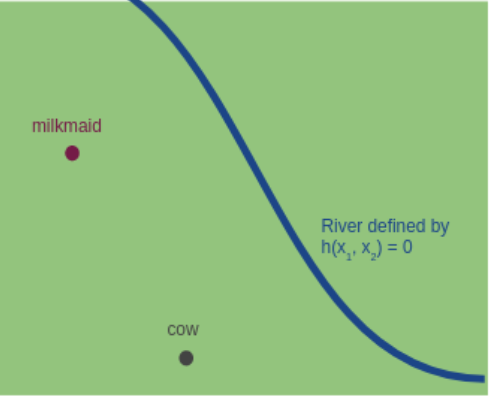
\includegraphics[width = 0.4\textwidth]{figure_man/milkmaid1.png}
\end{center}

\framebreak 

Let us put this into maths: The milkmaid wants to find the point $P$ at the riverbank for which the total distance $f(P)$ is a minimum, with

\begin{itemize} 
\item $f(P)$ being defined as $f(P) := d(M, P) + d(P, C)$ 
(distance from $M$ to $P$ + distance from $P$ point to $C$), and
\item the river is described by $h(x_1, x_2) = 0$. 
\end{itemize}

\begin{center}
	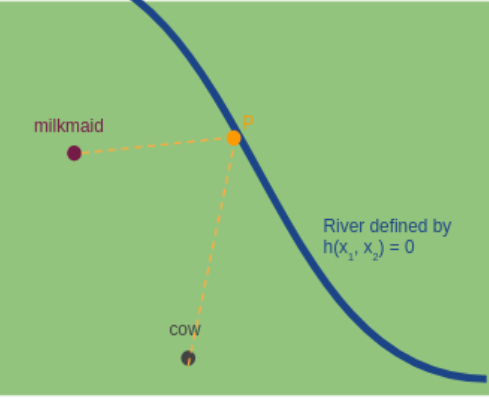
\includegraphics[width = 0.4\textwidth]{figure_man/milkmaid2.png}
\end{center}


\framebreak 

We want to solve the following optimization problem 

\begin{eqnarray*}
	\min_{x_1, x_2} && f(x_1, x_2) \\
	\text{s. t. } && h(x_1, x_2) = 0.
\end{eqnarray*}


\begin{center}
	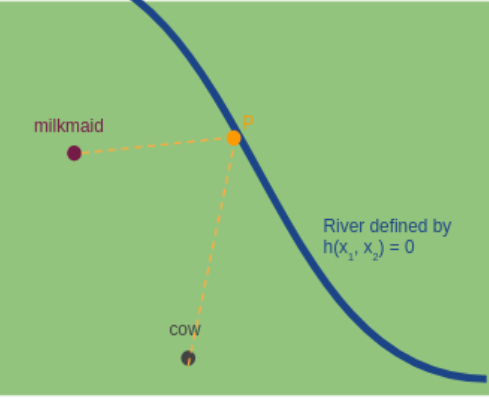
\includegraphics[width = 0.4\textwidth]{figure_man/milkmaid2.png}
\end{center}


\framebreak 

Let us visualize how far the milkmaid could get for any fixed total distance $f(P)$. 

\vspace*{0.2cm}

Let us first assume we only care about the distance from $M$ to $P$. We might picture this as a set of concentric circles. How far can the milkmaid get for a distance of $5$, $10$, $15$, ... meters?

\begin{center}
	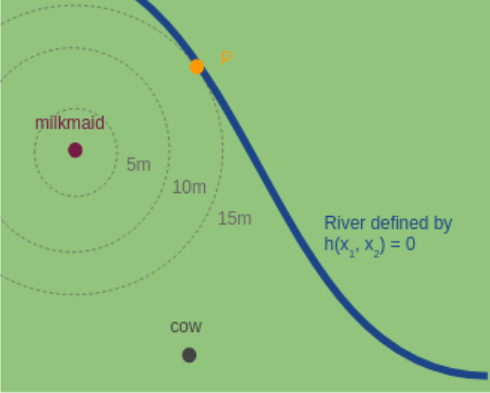
\includegraphics[width = 0.4\textwidth]{figure_man/milkmaid3.png}
\end{center}

As soon as one of those circles was big enough to touch the river, we'd recognize the point where it touched as the closest riverbank point to $M$. 

\framebreak 

We use now the geometric definition of an ellipse: 

Given two fixed points, $F_1$, $F_2$ called the foci and a distance $2a$ which is greater than the distance between the foci, the ellipse is the set of points $P$ such that the sum of the distances $|PF_1|, |PF_2|$ is equal to $2a$: 

$$
E = \{ P \in \mathbb{R}^2 | \, |PF_1| + |PF_2| = 2a \}
$$

\vspace*{0.2cm} 

\begin{center}
	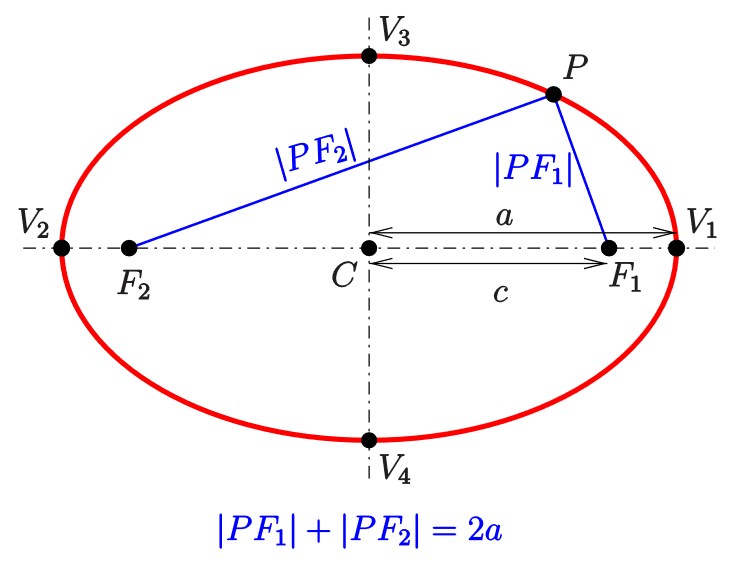
\includegraphics[width = 0.4\textwidth]{figure_man/ellipse.png}
\end{center}

\framebreak 

%Our problem is of course more difficult. However, we can make use of the following: For every point $P$ on a fixed ellipse with foci $M$ and $C$, the distance from $M$ to $P$ and back from $P$ to $C$ stays the same (independent of the exact choice of $P$). 



In the milkmaid problem, this means that the milkmaid could get to the cow by way of any point on a given ellipse with foci $M$ and $C$ in the same amount of time: the ellipses are curves of constant $f(P)$. 

\vspace*{0.2cm} 

\begin{center}
	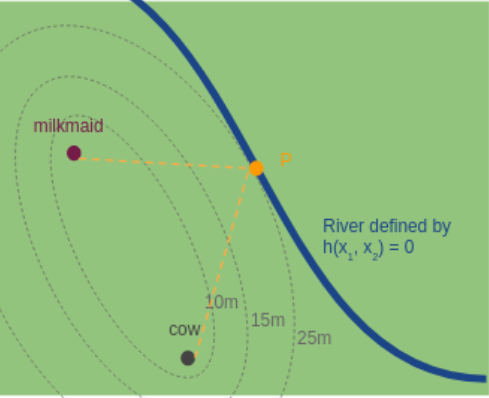
\includegraphics[width = 0.4\textwidth]{figure_man/milkmaid4.png}
\end{center}


\framebreak

Therefore, to find the desired point $P$ on the riverbank, we must simply find the \textbf{smallest ellipse} with $M$ and $C$ as foci, that intersects the curve of the river. 

\vspace*{0.2cm} 

The optimum point $P$ is the one where the respective ellipse is just \textbf{tangential} to the riverbank! 

\begin{center}
	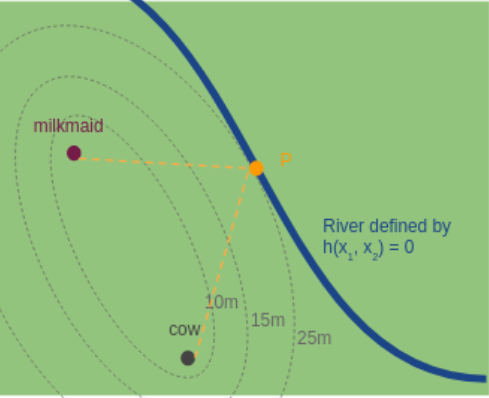
\includegraphics[width = 0.4\textwidth]{figure_man/milkmaid4.png}
\end{center}

It is obvious from the picture that the \enquote{perfect} ellipse and the river are truly tangential to each other at the ideal point $P$! 


\framebreak 

In multivariate calculus, the gradient $\nabla h$ of a function $h$ is normal to a surface on which $h$ is constant ($\nabla h$ is normal to the \enquote{contour lines}). 

\vspace*{0.2cm}

In our case, we have two functions whose normal vectors are parallel: 
$$
	\nabla f(P) = \beta \nabla h(P). 
$$

The multiplier $\beta$ is necessary because the magnitudes of the two gradients may be different. $\beta$ is called \textbf{Lagrange multiplier}. 

\begin{center}
	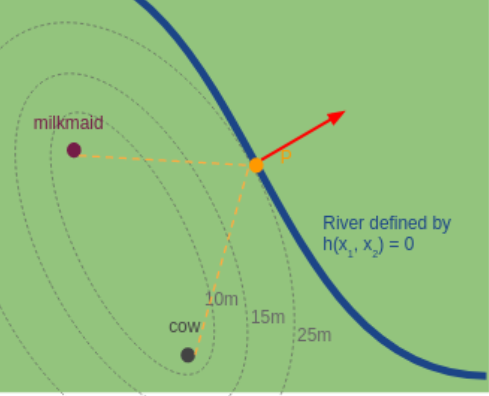
\includegraphics[width = 0.4\textwidth]{figure_man/milkmaid5.png}
\end{center}

\end{vbframe}

\begin{vbframe}{Lagrange Function}

In order to solve a problem with a single equality constraint, we require the following to be fulfilled: 

\begin{eqnarray*}
\nabla f(\xv^\ast) &=& \beta \nabla h(\xv^\ast), \quad \beta \in \R\\
h(\xv^\ast) &=& 0
\end{eqnarray*}

where the first line requires that gradients are parallel, and the second requires that the constraint is met. 

\lz 

This can also be written as: 

\begin{eqnarray*}
\nabla f(\xv^\ast) + \beta \nabla h(\xv^\ast) &=& 0, \quad \beta \in \R\\
h(\xv^\ast) &=& 0
\end{eqnarray*}

\framebreak 

If we define $\mathcal{L}(\xv, \beta) := f(\xv) + \beta h(\xv)$, then the point fulfilling the equations above is nothing but a stationary point of $\mathcal{L}$: 

$$
  \begin{pmatrix}
  \nabla_\xv \mathcal{L}(\xv^\ast, \beta) \\
  \nabla_\beta \mathcal{L}(\xv^\ast, \beta)
  \end{pmatrix} = \begin{pmatrix} \nabla f(\xv^\ast) + \beta \nabla h(\xv^\ast) \\
  h(\xv)
  \end{pmatrix} = \begin{pmatrix}
  0 \\ 0 \end{pmatrix}
$$

The function $\mathcal{L}$ is called \textbf{Lagrange function} or \textbf{Lagrangian}. 

\vspace*{0.2cm}

Note: In some books the Lagrangian is defined as $\mathcal{L}(\xv, \beta) := f(\xv) - \beta h(\xv)$. Both conventions obtain the same stationary points, but the sign of $\beta$ is different. 

\framebreak

The method can be extended to inequality constraints of the form $g(\xv) \geq 0$. There are two possible cases for a solution: 

\begin{itemize}
	\item If the optimal solution $x_b$ is inside the constraint region, the constraint is inactive, meaning that $\beta$ can be set to zero. 
	\item If the optimal solution $x_a$ lies on the boundary $g(\xv) = 0$, the negative gradient $\nabla f$ points in the opposite direction of the gradient of $g(\xv)$
\end{itemize}

\begin{center}
	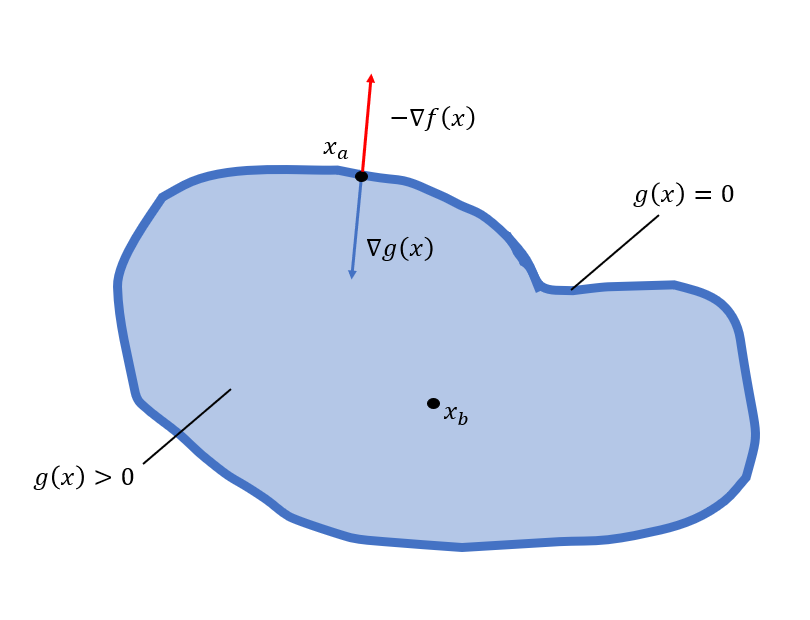
\includegraphics[width = 0.4\textwidth]{figure_man/constraint_lagrange.png}
\end{center}
\end{vbframe}




% \begin{vbframe}{Lagrange function: geometry}

% We imagine the contour lines of $f(\xv) = -2 + x_1^2 + 2 x_2^2$ as a \enquote{balloon} that is inflated. The higher the value of the function, the more the balloon is inflated.

% \vspace*{-0.5cm}

% <<echo = F, fig.width = 6, fig.asp = 1, fig.align = 'center', out.width = '50%'>>=
% source("rsrc/lagrange.R")

% x = seq(- 1.2, 1.2, by = 0.01)
% y = seq(- 1.2, 1.2, by = 0.01)
% z = outer(x, y, function(x1, x2) - 2 + x1^2 + 2 * x2^2)

% lagrangeContour()
% @

% \framebreak

% We include the precondition $x_1^2 + x_2^2 - 1 = 0$.

% \vspace*{-0.5cm}

% <<echo = F, fig.width = 6, fig.asp = 1, fig.align = 'center', out.width = '60%'>>=
% h.x1 = seq(-1, 1, length.out = 100)
% h.x2 = c(- sqrt(1 - h.x1[1:50]^2), - sqrt(1 - h.x1[51:100]^2), sqrt(1 - h.x1[100:51]^2), sqrt(1 - h.x1[50:1]^2))
% h.x1 = c(h.x1[1:50], h.x1[51:100], h.x1[100:51], h.x1[50:1])

% h.y = h.x1^2 + h.x2^2

% p1 = c(- sqrt(0.5), - sqrt(0.5))
% p2 = c(-1, 0)

% seq.along = seq(- sqrt(0.5), -1, length.out = 20)
% path = as.data.frame(matrix(c(seq.along, - sqrt(1 - seq.along^2)), ncol = 2))
% colnames(path) = c("x", "y")

% lagrangeContour(constraint = T, add.path = T)
% @


% \framebreak

% \begin{itemize}
% \item If the \enquote{balloon} is too small, the precondition is not yet fulfilled (e.g. for $f(\xv) = - 1.5$) and we inflate the balloon further.
% \item The same is true if the balloon is too big. Air must be released from the balloon.
% \item For $f(\xv) = - 0.5$ the constraint is fulfilled, because the contour line and the constraint intersect.
% \item However, points \enquote{within} the contour line $f(\xv) = - 0.5$ have smaller function values. So we could get better by letting some air out of the balloon.
% \item This works until the \enquote{balloon} and the precondition just touch, i.e. they are \textbf{tangential} to each other. This applies for $f(\xv) = -1$.
% \end{itemize}

% \framebreak

% The fact that the contour line and the precondition are \textbf{tangential} to each other in the optimum $\xv^*$ is equivalent to the fact that the respective \textbf{gradients} run parallel to each other.

% \vspace*{-0.3cm}
% \begin{eqnarray*}
% - \nabla f(\xv^*) = \beta \nabla h(\xv^*)
% \end{eqnarray*}

% Of course, we still demand that the precondition is fulfilled, i.e. that

% \vspace*{-0.3cm}
% \begin{eqnarray*}
% h(\xv^*) = 0.
% \end{eqnarray*}

% These can be combined to the \textbf{Lagrange} function with Lagrange multiplier~$\beta$:

% $$
% \mathcal{L}(\xv, \beta) := f(\xv) + \beta h(\xv).
% $$

% \vspace*{0.3cm}

% We are now looking for \textbf{stationary points} of the Lagrange function:

% $$
%   \begin{pmatrix}
%   \nabla_x \mathcal{L}(\xv^*, \beta) \\
%   \nabla_\beta \mathcal{L}(\xv^*, \beta)
%   \end{pmatrix} = \begin{pmatrix} \nabla f(\xv^*) + \beta \nabla h(\xv^*) \\
%   h(\xv)
%   \end{pmatrix} = \begin{pmatrix}
%   0 \\ 0 \end{pmatrix}
% $$

% \framebreak

% For the above example, the Lagrange function is

% $$
% \mathcal{L}(x_1, x_2, \beta) := -2 + x_1^2 + 2x_2^2 + \beta (x_1^2 + x_2^2 - 1).
% $$

% We set the gradient to $0$

% $$
% \nabla \mathcal{L}(x_1, x_2, \beta) = \begin{pmatrix} \frac{\partial{L}}{\partial{x_1}} \\ \frac{\partial{L}}{\partial{x_2}} \\ \frac{\partial{L}}{\beta} \end{pmatrix} = \begin{pmatrix} 2x_1 + 2 \beta x_1 \\ 4x_2 + 2 \beta x_2 \\ x_1^2 + x_2^2 - 1 \end{pmatrix} = 0
% $$

% and see that either $\beta = -1$ or $\beta = - 2$ must apply.

% \begin{itemize}
% \item For $\beta = -1$: $x_2 = 0$ and $x_1 = \pm 1$ (as already calculated).
% \item For $\beta = -2$: $x_2 = \pm 1$ and $x_1 = 0$.
% \end{itemize}

% These are the maxima / minima of the function.

% \end{vbframe}


\begin{vbframe}{Lagrange function and primal problem}

The Lagrangian can be extended to general constrained optimization problems with $k$ inequality constraints ($g(\xv) \geq 0$) and $l$ equality constraints ($g(\xv) = 0$): 

$$
\mathcal{L}(\xv, \bm{\alpha}, \bm{\beta}) := f(\xv) + \sum_{i=1}^k \alpha_i g_i(\xv) + \sum_{j=1}^l \beta_j h_j(\xv)
$$

with \textbf{Lagrange multipliers} $\alpha_i\ge 0$, $\beta_i$.

\lz

We can write the problem \textbf{equivalently} as

$$
\min_{\xv} \max_{\bm{\alpha}\ge 0, \bm{\beta}}  \mathcal{L}(\xv, \bm{\alpha}, \bm{\beta}).
$$

We call this problem \textbf{primal problem}. \\

\vspace*{0.2cm} 

Why is the above formulation equal to our initial (constrained) formulation of the optimization problem? 

\framebreak 

For simplicity, assume we only have a single inequality constraint. 

\vspace*{0.2cm} 

Assume an $\xv$ \textbf{does break} the inequality constraint, i.e., $g(\xv) > 0$. Then 

\vspace*{-0.5cm} 

\begin{eqnarray*}
	\max_{\alpha \ge 0} \mathcal{L}(\xv, \bm{\alpha}) = \max_{\alpha \ge 0} f(\xv) +  \alpha g(\xv) = \infty,
\end{eqnarray*}

because we can pick $\alpha = \infty$ to drive the objective value to infinity. 

\vspace*{0.2cm} 

If otherwise $g(\xv) \le 0$, 

\vspace*{-0.5cm} 

\begin{eqnarray*}
	\max_{\alpha \ge 0} \mathcal{L}(\xv, \bm{\alpha}) = \max_{\alpha \ge 0} f(\xv) +  \alpha g(\xv) = f(\xv),
\end{eqnarray*}

because $\alpha g(\xv) \le 0$ for any $\alpha \ge 0$, and $g(\xv) = 0$ if $\alpha = 0$. 

\framebreak 

We end up with 

\begin{eqnarray*}
	\min_x\max_{\alpha \ge 0} \mathcal{L}(\xv, \bm{\alpha}) = \begin{cases} \infty & \text{if } g(\xv) > 0 \\ \min_x f(\xv) & \text{if }  g(\xv) \le 0\end{cases}
\end{eqnarray*}

which corresponds to our original formulation. 

\vspace*{0.2cm} 

A similar argument holds for the equality constraint $h(\xv)$.

\end{vbframe}



\begin{vbframe}{Example: Lagrange function for QP's}


We consider quadratic programming

\begin{eqnarray*}
\min_{\xv} && f(\xv) := \frac{1}{2} \xv^\top \bm{Q} \xv \\
\text{such that} && h(\xv) := \bm{C} \xv - \bm{d} = 0,
\end{eqnarray*}

with $\bm{Q} \in \R^{d\times d}$ symmetric, $\bm{C} \in \R^{l \times d}, \bm{d} \in \R^n$.

\lz

The Lagrange function is

$$
\mathcal{L}(\xv, \bm{\beta}) = \frac{1}{2} \xv^\top \bm{Q} \xv + \bm{\beta}^\top \left(\bm{C} \xv - \bm{d}\right).
$$

\framebreak

For the calculation of the stationary points we calculate the gradient of the Lagrange function:

$$
\nabla \mathcal{L}(\xv, \bm{\beta}) = \begin{pmatrix} \frac{\partial{L}}{\partial{\xv}}  \\ \frac{\partial{L}}{\partial{\bm{\beta}}} \end{pmatrix} = \begin{pmatrix} \bm{Qx} + \bm{C}^\top\bm{\beta} \\ \bm{Cx - \bm{d}} \end{pmatrix} = \bm{0}
$$

This is a linear system with $n + p$ equations, which we write as

$$
\begin{pmatrix} \bm{Q} & \bm{C}^\top \\ \bm{C} & \bm{0} \end{pmatrix} \begin{pmatrix} \xv \\ \bm{\beta} \end{pmatrix} = \begin{pmatrix} \bm{0} \\ \bm{d}  \end{pmatrix}.
$$

It follows that finding stationary points of the Lagrange function corresponds to the solution of a system of linear equations and can be solved efficiently and stable with the help of suitable matrix decompositions (see chapter 7).
\end{vbframe}

\begin{vbframe}{Example: Lagrange function for Lasso}

\textbf{Lasso regression}: 

\begin{eqnarray*}
	\min_\theta && \|\yv - \Xmat \thetab\|_2^2 \\
	\text{s.t. } && \|\thetab\|^2_1 - t \le 0.
\end{eqnarray*}

We formulate the primal problem with the help of the Lagrangian:

\begin{eqnarray*}
	\min_\theta \max_{\alpha \ge 0} \mathcal{L}(\xv, \bm{\alpha}) &=& \min_\theta \max_{\alpha \ge 0} \left\{\|\yv - \Xmat \thetab\|_2^2 + \alpha \left(\|\thetab\|^2_1 - t\right)\right\}.
\end{eqnarray*}


\end{vbframe}


\begin{vbframe}{Lagrange duality}

The \textbf{dual problem} of the above problem results when we reverse minimization and maximization:

$$
\max_{\bm{\alpha} \ge 0, \bm{\beta}} \min_{\xv}  \mathcal{L}(\xv, \bm{\alpha}, \bm{\beta})
$$

We define the \textbf{dual function} $g(\bm{\alpha}, \bm{\beta}) := \min_{\xv}  \mathcal{L}(\xv, \bm{\alpha}, \bm{\beta})$.

\lz

We hold $\bm{\alpha}$ and $\bm{\beta}$ constant and optimize $\xv$ (unconstrained optimization problem!). In a second step, we maximize $\bm{\alpha}, \bm{\beta}$.

\lz

\textbf{Note:} This definition of duality is a generalization of the duality for Linear programming. For LPs, the two definitions are the same.

% Warum ist das Problem häufig einfacher zu lösen als andersherum?
% \begin{itemize}
% \item Die duale $g(\bm{\alpha}, \bm{\beta})$ hat häufig eine schöne, geschlossene Form.
% \item Im Gegensatz zur primalen Funktion ist $g(\bm{\alpha}, \bm{\beta})$ i.d.R. stetig.
% \end{itemize}

\framebreak

Important characteristics of the dual problem:

\begin{itemize}
\item The dual problem is \textbf{always convex}. Many methods are therefore based on the solution of the dual problem.
\item \textbf{Weak duality} \textbf{always} applies, i.e.

$$
g(\bm{\alpha}^*, \bm{\beta}^*) \le f(\xv^*)
$$
\item If the primal problem is convex, we have \textbf{strong duality} in general$^{(1)}$, i.e.

$$
g(\bm{\alpha}^*, \bm{\beta}^*) = f(\xv^*)
$$
\end{itemize}

\vfill

\begin{footnotesize}
$^{(1)}$ \textbf{slater's condition} must be fulfilled. Read more here \url{http://www.cs.cmu.edu/~ggordon/10725-F12/slides/15-duality.pdf}.
\end{footnotesize}

\end{vbframe}






%\begin{vbframe}{Optimalitätsbedingungen}


% Für einen Punkt $\xv \in \mathcal{S}$ definieren wir die Indexmenge der aktiven Ungleichungsnebenbedingungen
%
% $$
% \mathcal{A}(\xv) = \{i: 1 \le i \le m: g_i(\xv) = 0\}.
% $$
%
% Die Menge $\mathcal{A}(\xv)$ beschreibt also, welche Ungleichungen mit Gleichheit erfüllt sind.
%
% \framebreak
%
% \textbf{Frage: } Ist $\nabla \mathcal{L}(\xv^*, \beta) = 0$ eine \textbf{notwendige Optimalitätsbedingung}?
%
% \lz
%
% Im Gegensatz zur unrestringierten Optimierung, ist die Formulierung hinreichender und notwendiger Optimalitätsbedingungen komplizierter. Wir müssen berücksichtigen, dass wir uns möglicherweise am Rand des zulässigen Bereiches befinden.

% \lz
%
% Wir betrachten zunächst ein einfaches Beispiel
%
% \vspace*{-0.5cm}
%
%   \begin{eqnarray*}
%     \min\limits_{x_1, x_2} &  - x_1 - x_2 & \\
%     \text{s.t.} & x_1^2 + x_2^2 & = 1
%   \end{eqnarray*}
%
% \lz
%
% Wir lösen das Optimierungsproblem, indem wir die Zielgerade (also die Niveaulinie $f(\xv) = c$) so lange verschieben, bis wir einen Punkt finden, der die Nebenbedingung erfüllt und die Zielfunktion minimiert.
%
% \framebreak
%
% \center
%   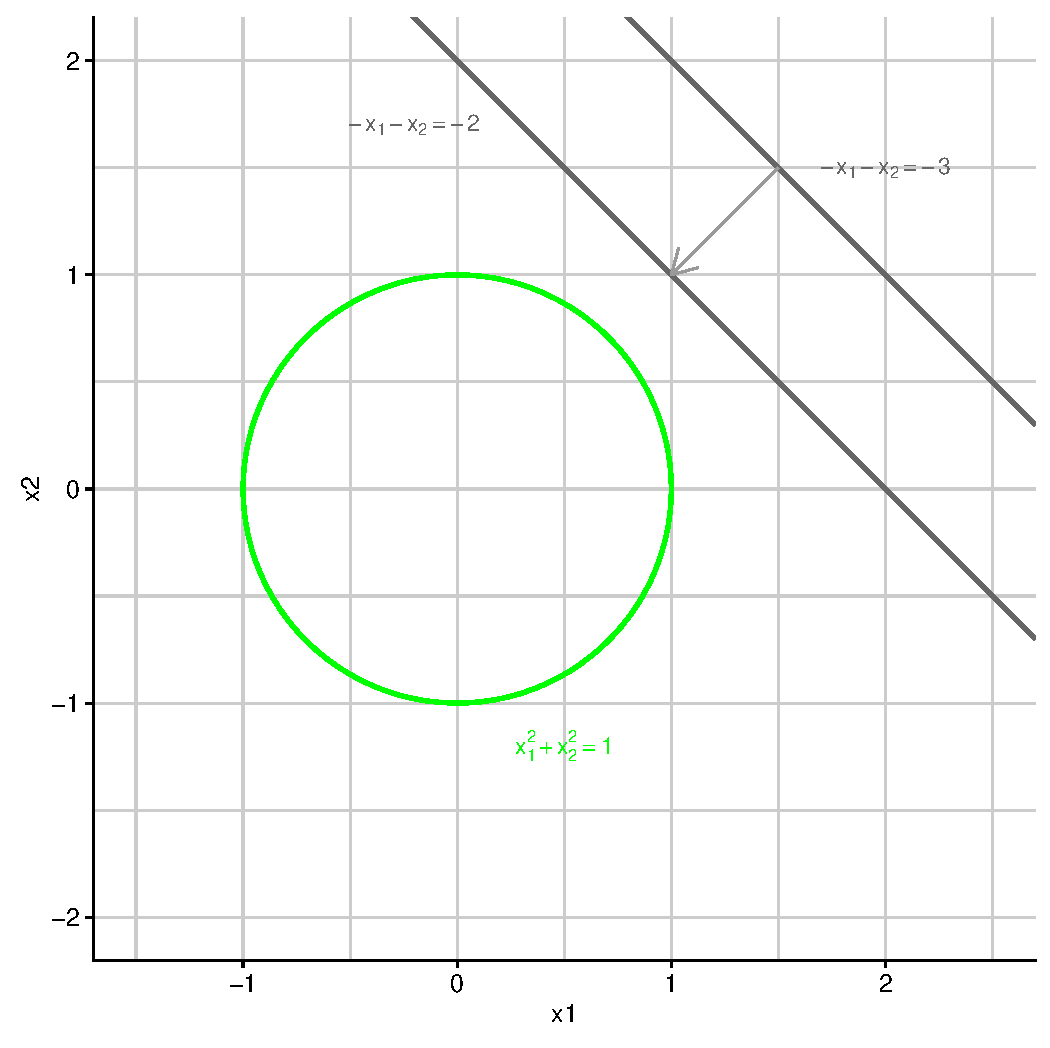
\includegraphics[width = 0.6\textwidth]{figure_man/constraints_violated.pdf}
%
% \framebreak
%
%   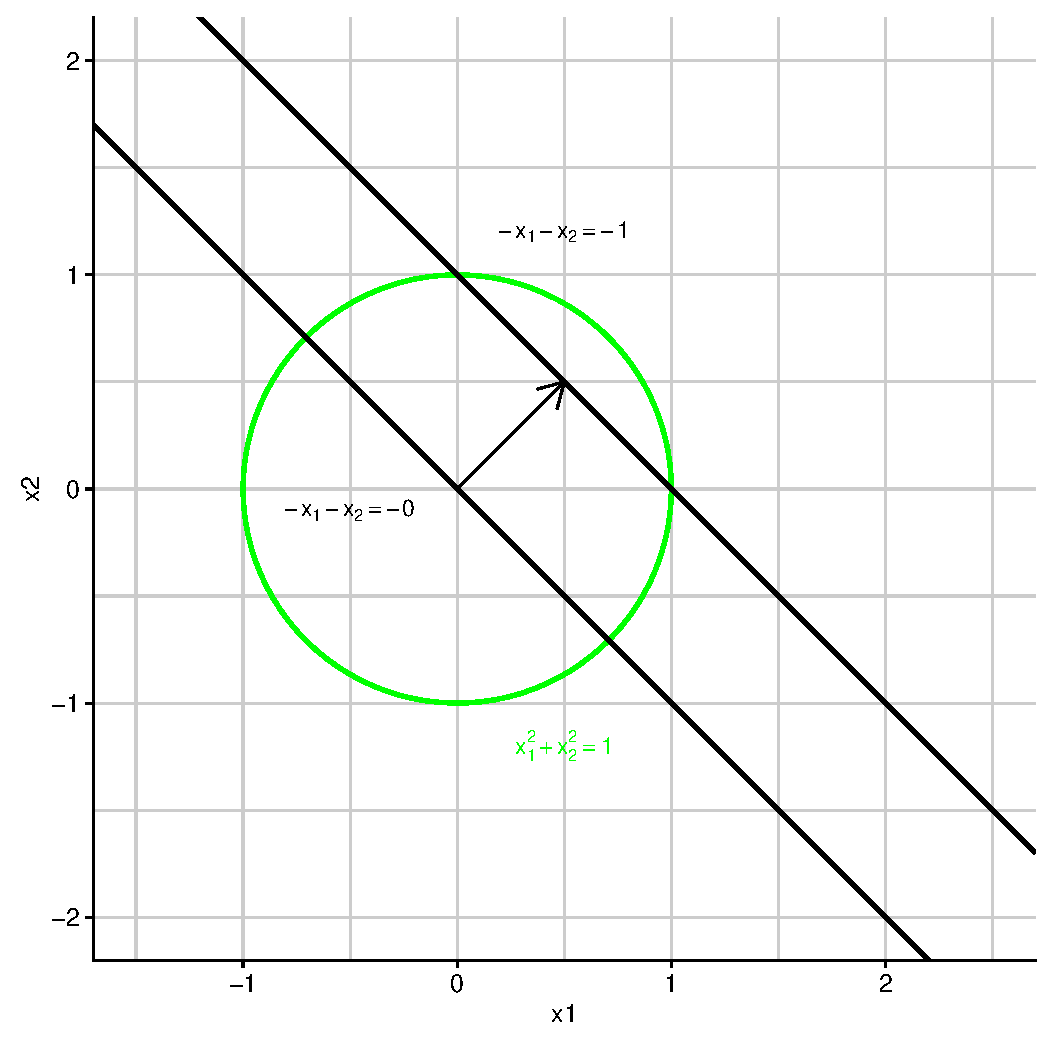
\includegraphics[width = 0.6\textwidth]{figure_man/constraints_satisfied.pdf}
%
% \framebreak
%
%   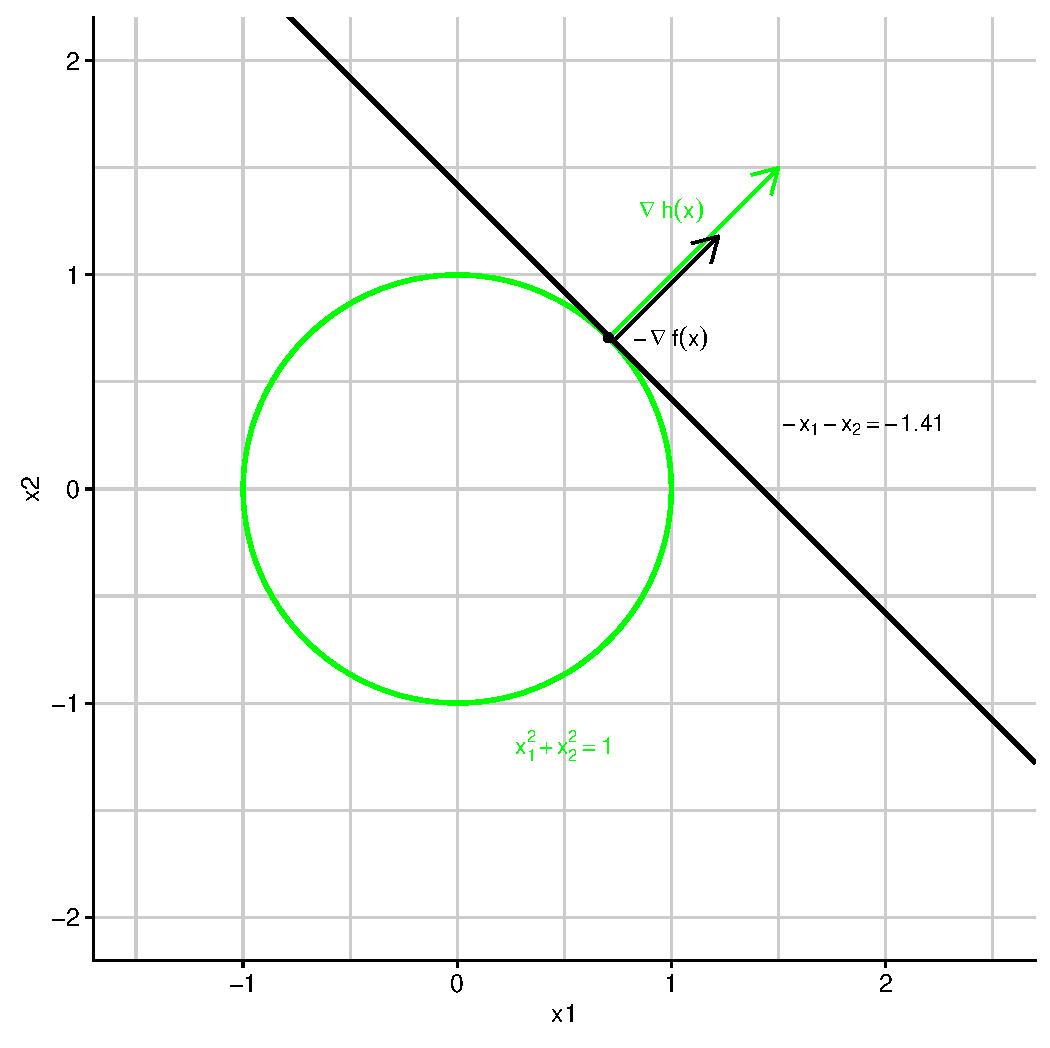
\includegraphics[width = 0.6\textwidth]{figure_man/constraints_opt.pdf}
%
% \framebreak
%
% \flushleft
%
% \textbf{Beobachtung}: Das Optimum $\xv^*$ ist genau dort, wo die Höhenlinie tangential zur Hyperebene der Nebenbedingung liegt.
%
% \lz
%
% In anderen Worten: $- \nabla f(\xv^*)$, $\nabla h(\xv^*)$ sind parallel.
%
% $$
%   - \nabla f(\xv^*) = \beta \nabla h(\xv^*)
% $$
%
% oder äquivalent
%
% $$
%   \nabla \mathcal{L}(\xv^*, \beta) := \nabla (f(\xv^*) + \beta h(\xv^*)) = \nabla f(\xv^*) + \nabla \beta h(\xv^*) = 0
% $$
%
%
% \lz
%
%
%
% \end{vbframe}

\endlecture
\end{document}



